\section{Auswertung}
\label{sec:Auswertung}
\subsection[Gamma-Strahlung]{$\gamma$-Strahlung}

Zunächst wird wie in \hyperref[sec:Durchführung]{Kapitel \ref{sec:Durchführung}} beschrieben eine Nullmessung durchgeführt werden.
Dabei ergibt sich bei einer Zeit von $t = 900 \unit\second$ eine Impulsrate von $N = 960 \pm 31$,
wobei sich der Fehler nach der Poissonverteilung richtet und somit durch $\increment N = \sqrt{N}$ berechnet wird.
Daraus erfolgt dann eine Aktivitätsrate von $A_0 = 1.07 \pm 0.034 \frac{1}{\unit\second}$, wobei der Fehler nach
der Formel in \autoref{eq:fehlerfortplanzung} berechnet wurde.

Nun soll der Absorptionskoeffizient von Blei und Kupfer bestimmt werden.

\subsubsection*{Absorptionskoeffizient von Blei}

Die Messdaten zu der Messung von Blei ist in \autoref{tab:md1blei} zu finden.
Logarithmisch aufgetragen sind die Messdaten und der Fit in \autoref{fig:plot1} zu finden.
Daraus ergeben sich auch der experimentell ermittelte Absorptionskoeffizient, welcher als Betrag der negativen Steigung der Geraden approximiert wird, und die Anfangsaktivität.
Diese sind
\begin{align*}
    \text{Absorptionskoeffizient:} && \mu &= (95.25 \pm 2.74) \frac{1}{\unit\meter},\\
    \text{Anfangsaktivität:} && A_0 &= (119.79 \pm 2.57) \frac{1}{\unit\meter}.
\end{align*} 
Wird nun der Wirkungsquerschnitt über \autoref{eq:Compton} mit $\epsilon = 1-295$ berechnet,
folgt mit $M_\text{Blei} = 207.2 \unit{\gram\mol^{-1}}$ \cite{molaremasse} und $ \rho_\text{Blei} = 11.34 \unit{\gram\centi\meter^{-3}}$
\begin{equation}
    \mu_\text{Theorie} = 69.34 \frac{1}{\unit\meter}.
\end{equation}


\begin{figure}
    \centering
    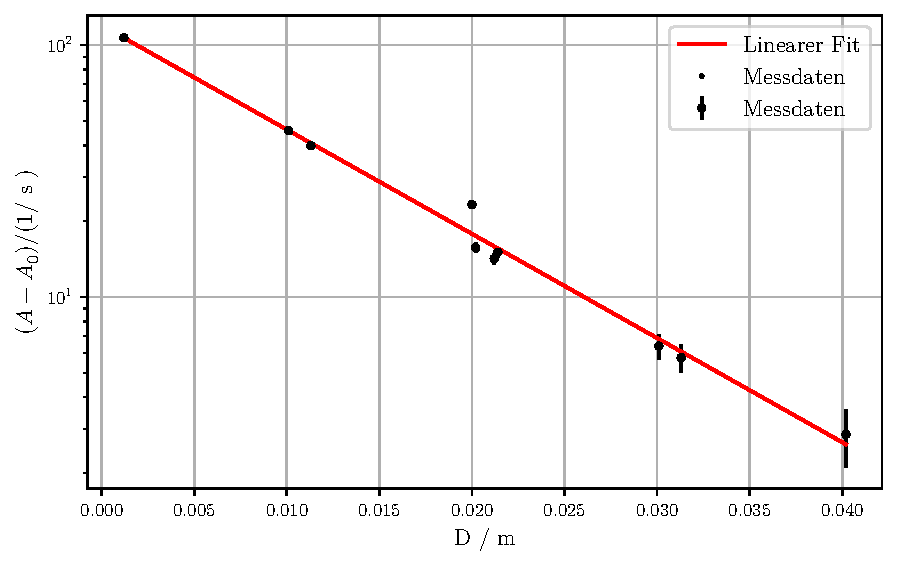
\includegraphics[width=0.7 \linewidth]{build/plot1.pdf}
    \caption{Gemessene Impulsrate bei unterschiedlichen Absorberdicken von Blei.}
    \label{fig:plot1}
\end{figure}


\begin{table}[H]
    \centering
    \caption{Messdaten des Absorptionskoeffizienten für Blei}
    \label{tab:md1blei}
    \begin{tabular}{c c c c}
        \toprule
        $d / \unit{\milli\meter}$ &  $t / \unit\second$ &     n & $A(D) - A_0 \frac{1}{\unit\second}$\\ 
        \midrule
            1,2 &  200 & 21610 $\pm$ 150 &  107.0 $\pm$ 0.7 \\
           10,1 &  200 &  9360 $\pm$ 100 &   45.7 $\pm$ 0.5 \\
           11,3 &  200 &  8190 $\pm$ 90  &   39.9 $\pm$ 0.5 \\
           20,0 &  300 &  7300 $\pm$ 90  & 23.28  $\pm$ 0.28 \\
           21,4 &  300 &  4840 $\pm$ 70  & 15.06  $\pm$ 0.23 \\
           30,1 &  400 &  2980 $\pm$ 60  &  6.39  $\pm$ 0.14 \\
           31,3 &  400 &  2730 $\pm$ 50  &  5.75  $\pm$ 0.13 \\
           21,2 &  400 &  6110 $\pm$ 80  & 14.22  $\pm$ 0.20 \\
           20,2 &  400 &  6710 $\pm$ 80  & 15.70  $\pm$ 0.21 \\
           40,2 &  500 &  1960 $\pm$ 40  &  2.85  $\pm$ 0.09 \\
        \bottomrule
    \end{tabular}
\end{table}

\subsubsection*{Absorptionskoeffizient von Kupfer}

Analog zu Blei wird nun auch für Kupfer der Absorbtionskoeffizient bestimmt.
Die entsprechenden Messdaten sind in \autoref{tab:md2kupfer} notiert und der Plot sowie der Fit sind in \autoref{fig:plot2} aufgetragen.
Aus der Ausgleichsrechnung ergeben sich dann die Werte
\begin{align*}
    \text{Absorbtionskoeffizient:} && \mu &= (37.32 \pm 2.89) \frac{1}{\unit\meter},\\
    \text{Anfangsaktivität} && A_0 &= (114.11 \pm 2.17) \frac{1}{\unit\meter}.
\end{align*} 
Nun wird auch der theoretische Wirkungsquerschnitt von Kupfer berechnet.
Mit $M_\text{Blei} = 63.55 \unit{\gram\mol^{-1}}$ \cite{molaremasse} und $ \rho_\text{Blei} = 8.95 \unit{\gram\centi\meter^{-3}}$ folgt
\begin{equation}
    \mu_\text{Theorie} = 63.1 \frac{1}{\unit\meter}.
\end{equation}


\begin{figure}
    \centering
    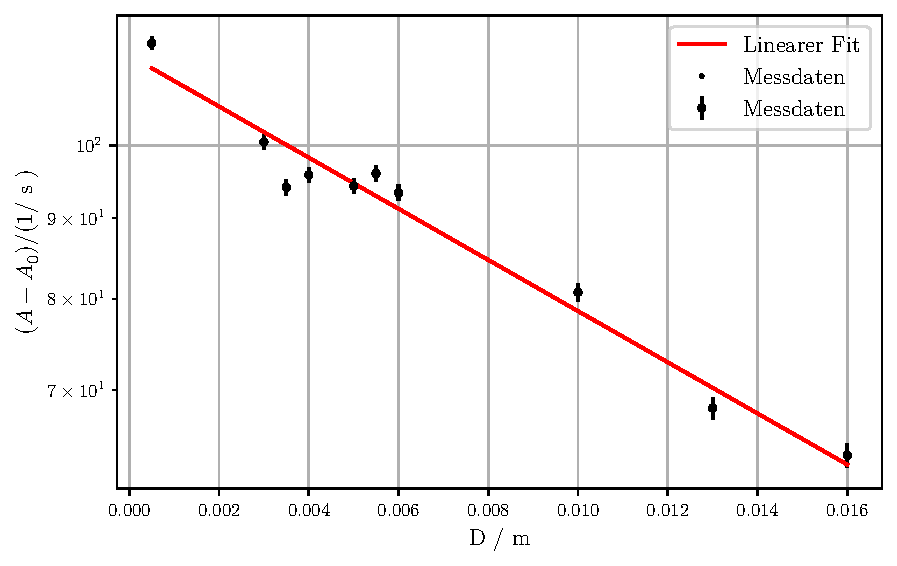
\includegraphics[width=0.7 \linewidth]{build/plot2.pdf}
    \caption{Gemessene Impulsrate bei unterschiedlichen Absorberdicken von Kupfer.}
    \label{fig:plot2}
\end{figure}

\begin{table}[H]
    \centering
    \caption{Messdaten des Absorptionskoeffizienten für Kupfer}
    \label{tab:md2kupfer}
    \begin{tabular}{c c c c}
        \toprule
        $d / \unit{\milli\meter}$ &  $t / \unit\second$ &     n & $A(D) - A_0 \frac{1}{\unit\second}$\\
        \midrule
            0,5 &    100 & 11720 $\pm$ 110 & 116.1 $\pm$ 1.1 \\
            3,0 &    100 & 10160 $\pm$ 100 & 100.6 $\pm$ 1.0 \\
            3,5 &    100 &  9520 $\pm$ 100 &  94.1 $\pm$ 1.0 \\
            4,0 &    100 &  9690 $\pm$ 100 &  95.9 $\pm$ 1.0 \\
            5,0 &    150 & 14300 $\pm$ 120 &  94.3 $\pm$ 0.8 \\
            5,5 &    150 & 14560 $\pm$ 120 &  96.0 $\pm$ 0.8 \\
            6,0 &    150 & 14170 $\pm$ 120 &  93.4 $\pm$ 0.8 \\
           10,0 &    150 & 12270 $\pm$ 110 &  80.8 $\pm$ 0.7 \\
           13,0 &    200 & 13850 $\pm$ 120 &  68.2 $\pm$ 0.6 \\
           16,0 &    200 & 12950 $\pm$ 110 &  63.7 $\pm$ 0.6 \\
        \bottomrule
    \end{tabular}
\end{table}


\subsection[Beta-Strahlung]{$\beta$-Strahlung}

Bei diesem Aufbau wurde eine Impulsrate von 525 bei 900 s gewählt, woraus sich $A_0 = 0.583 \pm 0.025$ ergibt.
In \autoref{tab:md3alu} sind die Messwerte der Betastrahlung zu finden.
Diese sind in \autoref{fig:plot3} aufgetragen.
Dabei wurde wie in \autoref{fig:massenbelegung} die Regression in zwei Bereiche unterteilt.
Für die Regression wird der Ansatz
\begin{equation*}
    ln(A(D)) = a \cdot D + b
\end{equation*}
gewählt.
Der Schnittpunkt dieser beiden Regressionsgeraden ergibt dann den Wert für $R_\text{max}$.
Für die Regressionsgeraden ergeben sich die Werte:
\begin{align*}
    \text{Fit 1:}&\begin{cases}
    a_1= -0.69 &\pm 0.25 \\
    b_2= 0.38 &\pm 0.09 
    \end{cases}\\
    \text{Fit 2:}&\begin{cases}
    a_3= 78.74 &\pm 27.54\\
    b_4= 18.42 &\pm 4.17
    \end{cases}
\end{align*}
Daraus folgt dann mit
\begin{equation*}
    R_\text{max} = \frac{b_2 - b_1}{a_1 - a_2} = (0.23 \pm 0.1) \frac{\unit{\kilo\gram}}{\unit{\meter^2}} ,
\end{equation*}
woraus mit \autoref{eq:Emax} 
\begin{equation*}
    E_\text{max} = (0.62 \pm 0.2) \unit{\mega\eV}
\end{equation*}
folgt.
\begin{figure}
    \centering
    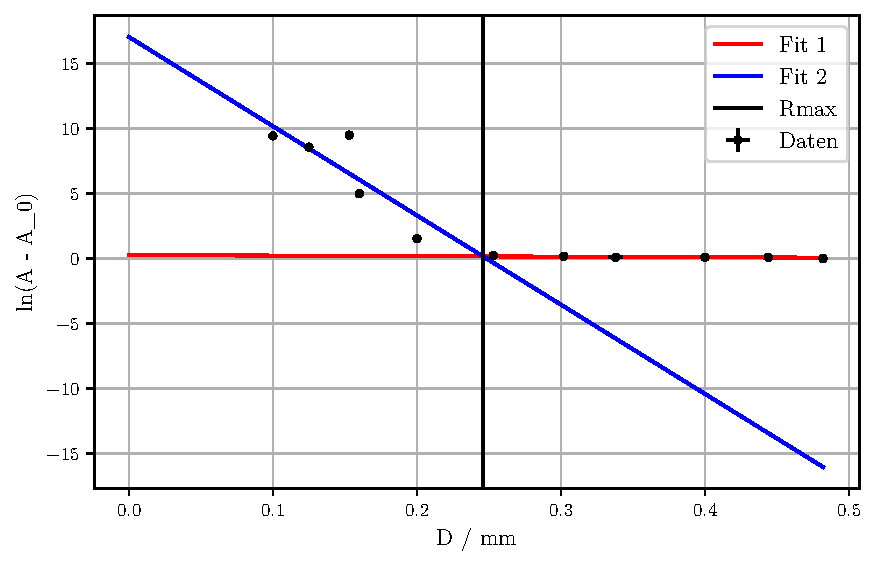
\includegraphics[width=0.7 \linewidth]{build/plot3.pdf}
    \caption{Gemessene Impulsrate bei unterschiedlichen Absorberdicken von Aluminium bei $\beta$-Strahlung.}
    \label{fig:plot3}
\end{figure}


\begin{table}
    \centering
    \caption{Messdaten des Absorptionskoeffizienten für Aluminium}
    \label{tab:md3alu}
    \begin{tabular}{c c c c}
        \toprule
        $d / \unit{\micro\meter}$ &  $t / \unit\second$ &     n & $A(D) - A_0 \frac{1}{\unit\second}$\\
        \midrule
                100 $\pm$ 0&    200 &   2000  $\pm$  40 &   9.42 $\pm$ 0.23 \\
                125 $\pm$ 0&    200 &   1830  $\pm$  40 &   8.57 $\pm$ 0.21 \\
                153 $\pm$ 0.5&    200 &   2010  $\pm$  40 &   9.49 $\pm$ 0.23 \\
                160 $\pm$ 1&    200 & 1113 $\pm$ 33 &   4.98 $\pm$ 0.17 \\
                200 $\pm$ 1&    400 &  843 $\pm$ 29 &   1.52 $\pm$ 0.07 \\
                253 $\pm$ 1&    400 &  325 $\pm$ 18 &   0.23 $\pm$ 0.04 \\
                302 $\pm$ 1&    400 &  302 $\pm$ 17 &   0.17 $\pm$ 0.04 \\
                338 $\pm$ 5&    500 &  337 $\pm$ 18 &   0.09 $\pm$ 0.04 \\
                400 $\pm$ 1&    500 &  339 $\pm$ 18 &   0.09 $\pm$ 0.04 \\
                444 $\pm$ 2&    500 &  340 $\pm$ 18 &   0.10 $\pm$ 0.04 \\
                482 $\pm$ 1&    500 &  297 $\pm$ 17 &   0.011$\pm$ 0.034\\
        \bottomrule
    \end{tabular}
\end{table}